\documentclass[tikz,border=6pt]{standalone}
\usepackage{pgfplots}
\pgfplotsset{compat=1.18}
\definecolor{demand}{HTML}{1F4E79}
\definecolor{mr}{HTML}{7EA6C8}
\definecolor{mc}{HTML}{B23A32}
\definecolor{ac}{HTML}{2F7D55}
\definecolor{point}{HTML}{C5161D}
\definecolor{profit}{HTML}{7BC99A}
\begin{document}
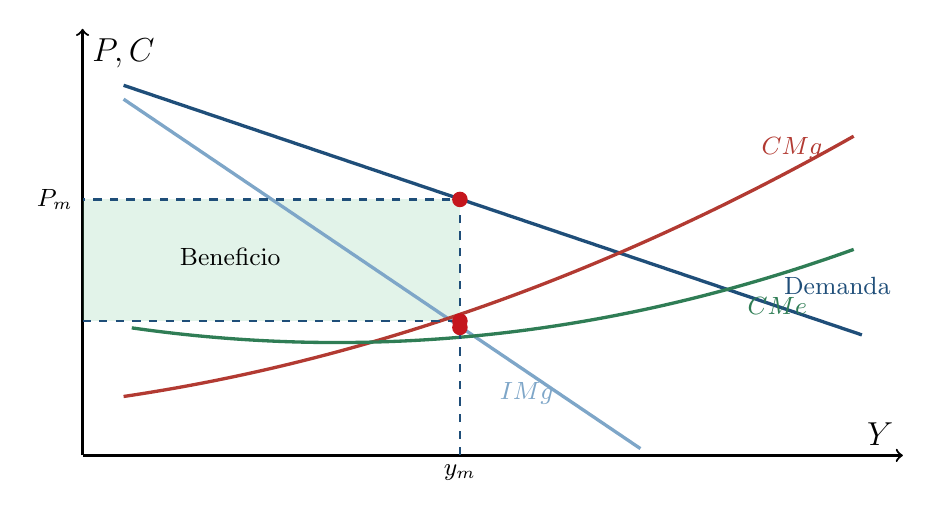
\begin{tikzpicture}
\begin{axis}[width=12cm,height=7cm,axis lines=middle,xmin=0,xmax=10,ymin=0,ymax=10,xtick=\empty,ytick=\empty,xlabel={$Y$},ylabel={$P,C$},axis line style={->,thick},label style={font=\large},tick style={draw=none},clip=false]
\path[fill=profit,opacity=.22] (axis cs:0,3.15) rectangle (axis cs:4.6,6.0);
\addplot[domain=.5:9.5,samples=2,very thick,demand] {9-.65*x} node[pos=.88,above right,font=\small] {Demanda};
\addplot[domain=.5:6.8,samples=2,very thick,mr] {9-1.3*x} node[pos=.78,below,font=\small] {$IMg$};
\addplot[domain=.5:9.4,samples=80,very thick,mc] {1.25+.24*x+.045*x^2} node[pos=.9,above,font=\small] {$CMg$};
\addplot[domain=.6:9.4,samples=100,very thick,ac] {2.25+.055*(x-4.1)^2+.11*x} node[pos=.82,below right,font=\small] {$CMe$};
\addplot[dashed,thick,demand] coordinates {(4.6,0) (4.6,6) (0,6)};
\addplot[dashed,thick,demand] coordinates {(0,3.15) (4.6,3.15)};
\addplot[only marks,mark=*,mark size=2.6pt,point] coordinates {(4.6,6) (4.6,3.15) (4.6,3.0)};
\node[left,font=\small] at (axis cs:0,6) {$P_m$};
\node[below,font=\small] at (axis cs:4.6,0) {$y_m$};
\node[font=\small] at (axis cs:1.8,4.65) {Beneficio};
\end{axis}
\end{tikzpicture}
\end{document}
